\documentclass[dvipsnames]{beamer}  

\mode<presentation>
{
  \usetheme{Singapore}
  % or ...
  \setbeamercovered{transparent}
  % or whatever (possibly just delete it)
}

\setbeamercolor{block body}{fg=black, bg=green!10}

\usepackage{fontspec} 
\usepackage[mathscr]{euscript} 
%\usepackage[xcharter]{newtxmath}
%\setmainfont{XCharter}
\setmonofont{DejaVu Sans Mono}[Scale=MatchLowercase] % provides unicode characters 


\usefonttheme{professionalfonts}
%\usepackage[english]{babel}
% or whatever
%\usepackage[latin1]{inputenc}
% or whatever
%\usepackage{times}
\usepackage[T1]{fontenc}
% Or whatever. Note that the encoding and the font should match. If T1
% does not look nice, try deleting the line with the fontenc.

%%%%%%%%%%%%%%%%%%%%%% start my preamble %%%%%%%%%%%%%%%%%%%%%%
\renewcommand{\insertnavigation}[1]{}

\addtobeamertemplate{navigation symbols}{}{%
    \usebeamerfont{footline}%
    \usebeamercolor[fg]{footline}%
    \hspace{1em}%
    \insertframenumber/\inserttotalframenumber
    \vspace{0.5em}
}

\setbeamercolor{footline}{fg=blue}
\setbeamerfont{footline}{series=\bfseries}

%\setbeamertemplate{mini frames}{}

%\usepackage{adjustbox}
\usepackage{graphicx}
\usepackage{amsmath, amssymb, amsthm}
\usepackage{mathtools}

\usepackage{fancyvrb}

\usepackage{hyperref}

\usepackage{mathrsfs} % fonts, caligraphic
\usepackage{bbm}

% tikz
\usepackage{tikz}
\usepackage{tikz-cd}
\usetikzlibrary{positioning}
\usetikzlibrary{arrows}
\usetikzlibrary{calc}
\usetikzlibrary{intersections}
\usetikzlibrary{matrix}
\usetikzlibrary{decorations}
\usetikzlibrary{shapes, fit}
\usetikzlibrary{arrows.meta}
\usetikzlibrary{decorations.pathreplacing}  %for brac

\usepackage{pgf}
\usepackage{pgfplots}
\pgfplotsset{compat=1.7}


\usepackage{graphviz}

%\usepackage[usenames, dvipsnames]{color}


% nice inequalities
\renewcommand{\leq}{\leqslant}
\renewcommand{\geq}{\geqslant}


\setlength{\parskip}{1.5ex plus0.5ex minus0.5ex}
\setlength{\jot}{12pt} 

\usepackage[ruled, lined]{algorithm2e}


\definecolor{pale}{RGB}{235, 235, 235}
\definecolor{pale2}{RGB}{175,238,238}
\definecolor{turquois4}{RGB}{0,134,139}
\definecolor{DarkOrange1}{RGB}{255,127,0}

\newcommand{\emp}[1]{\textcolor{DarkOrange1}{\bf #1}}
\newcommand{\newtopic}[1]{\textcolor{Green}{\Large \bf #1}}
\newcommand{\navy}[1]{\textcolor{Blue}{\bf #1}}
\newcommand{\navymth}[1]{\textcolor{Blue}{#1}}
\newcommand{\red}[1]{\textcolor{red}{#1}}

% Minted
\definecolor{bg}{rgb}{0.95,0.95,0.95}
\usepackage{minted}
\usemintedstyle{friendly}
\newminted{python}{mathescape,frame=lines,framesep=4mm,bgcolor=bg}
\newminted{ipython}{mathescape,frame=lines,framesep=4mm,bgcolor=bg}
\newminted{julia}{mathescape,frame=lines,framesep=4mm,bgcolor=bg}
\newminted{c}{mathescape,frame=lines,framesep=4mm,bgcolor=bg}
\renewcommand{\theFancyVerbLine}{\sffamily
    \textcolor[rgb]{0.5,0.5,1.0}{\scriptsize {\arabic{FancyVerbLine}}}}


\definecolor{Brown}{rgb}{0.59, 0.29, 0.0}
\newcommand{\Fact}{\textcolor{Brown}{\bf Fact. }}
\newcommand{\Thm}{\textcolor{Brown}{\bf Theorem. }}
\newcommand{\Eg}{\textcolor{ForestGreen}{Example. }}
\newcommand{\Egs}{\textcolor{ForestGreen}{Examples. }}
\newcommand{\Ex}{{\bf Ex. }}

\newcommand{\CC}{\mathbbm C}
\newcommand{\EE}{\mathbbm E}
\newcommand{\FF}{\mathbbm F}
\newcommand{\RR}{\mathbbm R}
\newcommand{\KK}{\mathbbm K}
\newcommand{\MM}{\mathbbm M}
\newcommand{\NN}{\mathbbm N}
\newcommand{\PP}{\mathbbm P}
\newcommand{\TT}{\mathbbm T}
\newcommand{\QQ}{\mathbbm Q}
\newcommand{\WW}{\mathbbm W}
\newcommand{\VV}{\mathbbm V}
\newcommand{\ZZ}{\mathbbm Z}

\newcommand{\Asf}{\mathsf A}
\newcommand{\Esf}{\mathsf E}
\newcommand{\Fsf}{\mathsf F}
\newcommand{\Gsf}{\mathsf G}
\newcommand{\Msf}{\mathsf M}
\newcommand{\Lsf}{\mathsf L}
\newcommand{\Nsf}{\mathsf N}
\newcommand{\Psf}{\mathsf P}
\newcommand{\Qsf}{\mathsf Q}
\newcommand{\Ssf}{\mathsf S}
\newcommand{\Tsf}{\mathsf T}
\newcommand{\Xsf}{\mathsf X}
\newcommand{\Ysf}{\mathsf Y}
\newcommand{\Vsf}{\mathsf V}
\newcommand{\Wsf}{\mathsf W}
\newcommand{\Zsf}{\mathsf Z}

\newcommand{\aA}{\mathscr A}
\newcommand{\bB}{\mathscr B}
\newcommand{\cC}{\mathscr C}
\newcommand{\dD}{\mathscr D}
\newcommand{\eE}{\mathscr E}
\newcommand{\gG}{\mathscr G}
\newcommand{\hH}{\mathscr H}
\newcommand{\iI}{\mathscr I}
\newcommand{\fF}{\mathscr F}
\newcommand{\lL}{\mathscr L}
\newcommand{\pP}{\mathscr P}
\newcommand{\rR}{\mathscr R}
\newcommand{\sS}{\mathscr S}
\newcommand{\vV}{\mathscr V}
\newcommand{\wW}{\mathscr W}
\newcommand{\mM}{\mathscr M}
\newcommand{\oO}{\mathscr O}
\newcommand{\zZ}{\mathscr Z}

\newcommand{\bP}{\mathbf P} 
\newcommand{\bR}{\mathbf R}
\newcommand{\bQ}{\mathbf Q}


%%%%%% special symbols %%%%%%%%%%

\newcommand{\volone}{Volume~I}
\newcommand{\voltwo}{Volume~II}

% transpose, not currently using
\newcommand\T{{\mathpalette\raiseT\intercal}}
\newcommand\raiseT[2]{\raisebox{0.25ex}{$#1#2$}}

% nice inequalities
\renewcommand{\leq}{\leqslant}
\renewcommand{\geq}{\geqslant}

% nice greek letters
\renewcommand{\phi}{\varphi}
\renewcommand{\epsilon}{\varepsilon}

% inner product
\providecommand{\inner}[1]{\left\langle{#1}\right\rangle}

% set of matrices
\newcommand{\matset}[2]{ \MM^{ #1 \times #2 } }

% stochastic dominance
\newcommand{\lefsd}{\preceq_{\textrm{F}}}
\newcommand{\lessd}{\preceq_{\textrm{S}}}

% argmax and min
\newcommand{\argmax}{\operatornamewithlimits{argmax}}
\newcommand{\argmin}{\operatornamewithlimits{argmin}}

% sets and logic
\newcommand{\st}{\ensuremath{\ \mathrm{s.t.}\ }}
\newcommand{\setntn}[2]{ \{ #1 : #2 \} }
\newcommand{\natset}[1]{[ #1 ]}

% some useful symbols
\newcommand{\given}{\, | \,}
\newcommand{\cf}[1]{ \lstinline|#1| }
\newcommand{\fore}{\therefore \quad}
\newcommand{\1}{\mathbbm 1}
\newcommand{\me}{\mathrm{e}}               % Euler's e
\newcommand*\diff{\mathop{}\!\mathrm{d}}   % d for integrals

% shortcuts
\newcommand{\la}{\langle}
\newcommand{\ra}{\rangle}

% relations
\newcommand{\eqdist}{\stackrel{d} {=} }
\newcommand{\iidsim}{\stackrel{\textrm{ {\sc iid }}} {\sim} }

% convergence
\newcommand{\tod}{\stackrel { d } {\to} }
\newcommand{\tow}{\stackrel { w } {\to} }
\newcommand{\toprob}{\stackrel { p } {\to} }
\newcommand{\toms}{\stackrel { ms } {\to} }


%%%%%%%%%%% operators %%%%%%%%%%%%

\DeclareMathOperator{\fix}{fix}  % exponential draw
\DeclareMathOperator{\Exp}{Exp}  % exponential draw
\DeclareMathOperator{\Lip}{Lip}
\DeclareMathOperator{\cl}{cl}
\DeclareMathOperator{\graph}{graph}
\DeclareMathOperator{\interior}{int}
\DeclareMathOperator{\Prob}{Prob}
\DeclareMathOperator{\determinant}{det}
\DeclareMathOperator{\trace}{trace}
\DeclareMathOperator{\sgn}{sgn}
\DeclareMathOperator{\Span}{span}
\DeclareMathOperator{\diag}{diag}
\DeclareMathOperator{\proj}{proj}
\DeclareMathOperator{\rank}{rank}
\DeclareMathOperator{\kernel}{null}
\DeclareMathOperator{\cov}{Cov}
\DeclareMathOperator{\corr}{Corr}
\DeclareMathOperator{\var}{Var}
\DeclareMathOperator{\mse}{mse}
\DeclareMathOperator{\se}{se}
\DeclareMathOperator{\range}{range}
\DeclareMathOperator{\dimension}{dim}
\DeclareMathOperator{\epi}{epi}
\DeclareMathOperator{\vecop}{vec}

\DeclareMathOperator{\real}{Re}
\DeclareMathOperator{\imag}{Im}

\DeclareMathOperator{\csum}{cs} % column sum
\DeclareMathOperator{\rsum}{rs} % row sum



\hypersetup{
    linkcolor=Blue,
    colorlinks=true,
    filecolor=magenta,      % color of file links
    urlcolor=cyan           % color of external links
}



\title{Dynamic Programming: \\ Theory and Computation}

\author{John Stachurski}

\date[\today]{}

\begin{document}

\begin{frame}
  \titlepage
\end{frame}


\begin{frame}
    \frametitle{Topics}

    \begin{itemize}
        \item DP problems
            \vspace{0.3em}
        \item DP theory
            \vspace{0.3em}
        \item DP algorithms 
    \end{itemize}

\end{frame}

\begin{frame}
    
    The focus of this lecture will be on 

    \begin{enumerate}
        \item core theory
        \item core algorithms and 
        \item numerical methods
    \end{enumerate}


\end{frame}


\begin{frame}
    
    For now we will stick to discrete problems

    \begin{itemize}
        \item finite action space $\Asf$
        \item finite state space $\Xsf$
    \end{itemize}

    On the other hand, we will allow many interesting features

    \begin{itemize}
        \item Epstein-Zin preferences
        \item state-dependent discounting
        \item risk-sensitive preferences
        \item quantile preferences
        \item nonlinear discounting, etc.
    \end{itemize}

\end{frame}


\begin{frame}{Prelude: some linear algebra}

    In what follows we sometimes need to deal with equations of the form

    \begin{equation*}
        v(x) = \sum_{x'} v(x') K(x, x') + b(x)
        \qquad (x \in \Xsf)
    \end{equation*}

    Here $K$ and $b$ are given, while $v$ is the unknown

    We think of $v$ is a function from finite set $\Xsf$ to $\RR$
    
    Our objective is to solve the equation for $v$

\end{frame}

\begin{frame}
    
    To make this simple we can think of this in terms of matrices and vectors

    Replacing $x = x_i$ with $i$, the equation

    \begin{equation*}
        v(x) = \sum_{x'} v(x') K(x, x') + b(x)
        \qquad \text{ for } x \in \Xsf
    \end{equation*}
    %
    becomes
    %
    \begin{equation*}
        v_i = \sum_{j} v_j K_{ij} + b_i
        \qquad \text{ for } i \in \{1, \ldots, n\}
    \end{equation*}

    or
    %
    \begin{equation*}
        v = K v + b
    \end{equation*}

\end{frame}

\begin{frame}[fragile]
    
    The spectral radius of $K$ is
    %
    \begin{equation*}
        r(K) \coloneq \max \setntn{|\lambda|}{\lambda \text{ is an eigenvalue of } K}
    \end{equation*}

    \medskip
    \medskip
    \medskip

    \begin{minted}{python}
import jax
import jax.numpy as jnp

@jax.jit
def spectral_radius(K):
    eigenvalues = jnp.linalg.eigvals(K)
    return jnp.max(jnp.abs(eigenvalues))
    \end{minted}

\end{frame}

\begin{frame}

   \Thm If $r(K) < 1$, then 
   %
   \begin{enumerate}
       \item $I-K$ is invertible with
           %
           \begin{equation*}
               (I-K)^{-1} = \sum_{i \geq 0} K^i
           \end{equation*}
           %
       \item and the equation $v = Kv + b$ has the unique solution 
           %
           \begin{align*}
               v^* & = (I - K)^{-1} b 
                   \\
                   & = \sum_{i \geq 0} K^i b
           \end{align*}
           %
   \end{enumerate}

   \medskip


   \textbf{Remark.} This is the matrix analogue of 
   %
   \begin{equation*}
       |a| < 1
       \quad \implies \quad
       \sum_{i \geq 0} a^i = \frac{1}{1-a}
   \end{equation*}

\end{frame}



\begin{frame}\frametitle{Introduction to DPs: the Affine Case}

    Consider a dynamic program with
    %
    \begin{enumerate}
        \item a finite set $\Xsf$ called the \navy{state space} and
        \vspace{0.5em}
        \item a finite set $\Asf$ called the \navy{action space}
    \end{enumerate}
     
    \vspace{0.5em}
        \vspace{0.5em}
        \vspace{0.5em}

    Actions are restricted by a \navy{feasible correspondence} $\Gamma$

    \begin{itemize}
        \vspace{0.5em}
        \item from $\Xsf$ to $\Asf$
        \vspace{0.5em}
        \item $\Gamma(x) =$ actions available in state $x$  (nonempty)
    \end{itemize}

\end{frame}


\begin{frame}

    The \navy{feasible state-action pairs} is the set
    %
    \begin{equation*}
        \Gsf := \setntn{(x, a) \in \Xsf \times \Asf}{a \in \Gamma(x)}
    \end{equation*}
    %

    
    The \navy{Bellman equation} takes the form
    %
    \begin{equation*}
        v(x)
        = \max_{a \in \Gamma(x)}
        \left\{
            r(x, a)
            + \sum_{x'} v(x') K(x, a, x')
        \right\}
    \end{equation*}

    Components:
    %
    \begin{itemize}
        \item the \navy{reward function} $r$ maps $\Gsf$ to $\RR$ and
        \item the \navy{transition kernel} $K$ maps $\Gsf \times \Xsf$ to $\RR$ 
    \end{itemize}

\end{frame}


\begin{frame}
    
    \Eg \navy{Job search}

    Set up:
        \vspace{0.5em}
    \begin{itemize}
        \item wage offer process $(W_t)_{t \geq 0}$ is $P$-Markov on finite set
            $\Wsf$: 
        \vspace{0.5em}
        %
        \begin{equation*}
            \text{$\PP\{W_{t+1} = w' \given W_t = w\} = P(w, w')$}
        \end{equation*}
        %
        \item discount factor $\beta \in (0,1)$
    \end{itemize}

        \vspace{0.5em}
        \vspace{0.5em}
    The Bellman equation is
    %
    \begin{equation*}
        v(w) =
        \max
        \left\{
            \frac{w}{1-\beta} , \,   c + \beta \sum_{w'} v(w') P(w, w')
        \right\}
    \end{equation*}

\end{frame}


\begin{frame}
    
    We can rewrite the Bellman equation as
    %
    \begin{equation*}
        v(w) =
        \max_{a \in \{0,1\}}
        \left\{
             a \frac{w}{1-\beta}  
             + (1-a) \left[ c + \beta \sum_{w'} v(w') P(w, w') \right]
        \right\}
    \end{equation*}
    %
    \medskip

    This is an affine DP with 
    %
    \begin{itemize}
        \item state $w \in \Wsf$
        \medskip
        \item $\Gamma(w) = \{0, 1\}$
        \medskip
        \item $r(w, a) = a w / (1-\beta) + (1-a)c$
        \medskip
        \item $K(w, a, w') = (1 - a) \beta P(w, w')$
    \end{itemize}

\end{frame}



\begin{frame}
    
    \Eg \navy{Firm exit}

    \medskip

    Firm observes current state of the world $z$ and decides whether to exit

    \begin{itemize}
        \item If exit then receive scrap value $s(z)$  
            \medskip
        \item If continue then receive profit $\pi(z)$
    \end{itemize}

    \medskip

    Set up:
    %
    \begin{itemize}
        \item state of the world $(Z_t)_{t \geq 0}$ is $P$-Markov on finite set $\Zsf$ 
            \medskip
        \item discount factor $\beta = 1/(1+r)$ with $r > 0$
    \end{itemize}

\end{frame}

\begin{frame}
    
    The Bellman equation is
    %
    \begin{equation*}
        v(z) =
        \max
        \left\{
            s(z) , \pi(z) + \beta \sum_{z'} v(z') P(z, z')
        \right\}
    \end{equation*}

    We can rewrite the Bellman equation as
    %
    \begin{equation*}
        v(z) =
        \max_{a \in \{0,1\}}
        \left\{
             a s(z)
             + (1-a) \left[ \pi(z) + \beta \sum_{z'} v(z') P(z, z') \right]
        \right\}
    \end{equation*}
    %
    \medskip

    This is also an affine DP

    %
    \begin{itemize}
        \item $r(z, a) = a s(z) + (1-a)\pi(z)$
        \medskip
        \item $K(z, a, z') = (1 - a) \beta P(z, z')$
    \end{itemize}

\end{frame}

\begin{frame}

    One limitation: constant discounting

    \medskip
    \medskip

    For this model we would expect
    %
    \begin{equation*}
        \beta = \frac{1}{1 + \text{interest rate}}
    \end{equation*}

    \vspace{0.4em}
    \vspace{0.4em}
    And interest rates vary over time

\end{frame}


\begin{frame}
    
    \begin{figure}
       \centering
       \scalebox{0.4}{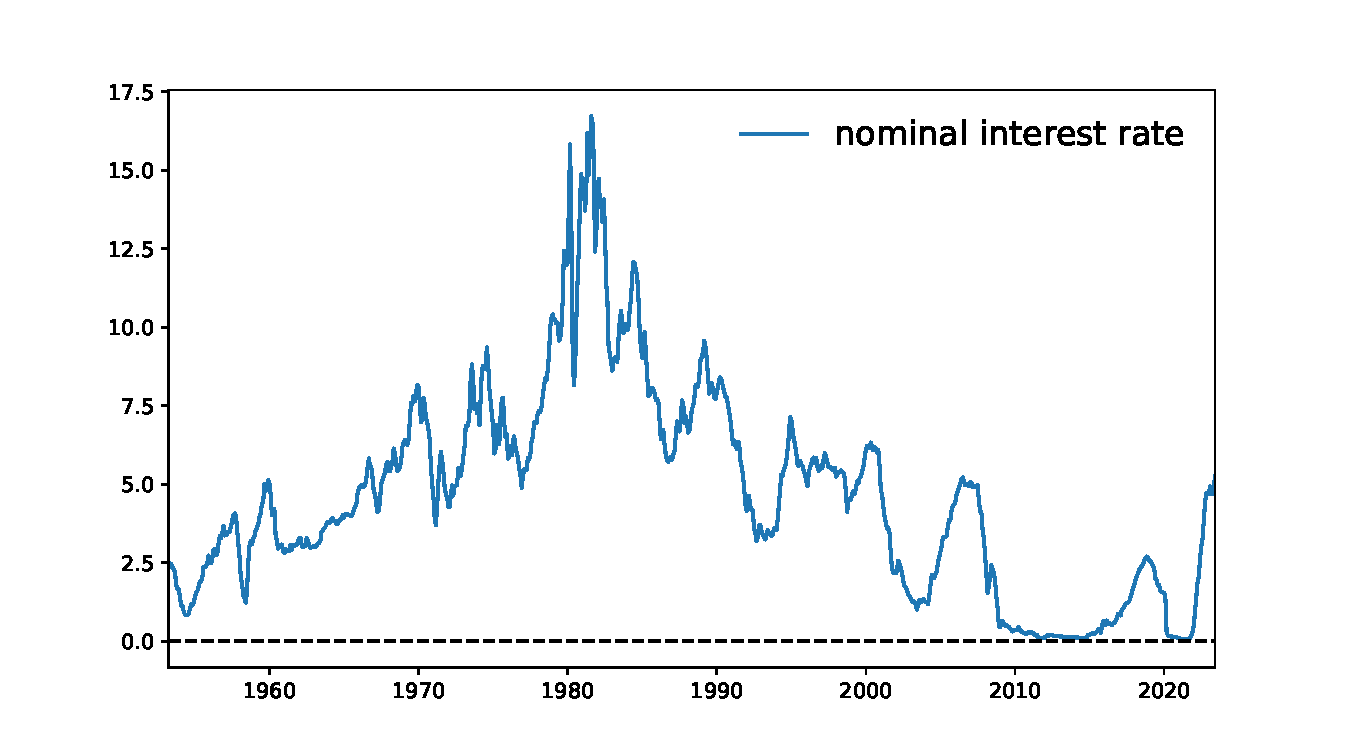
\includegraphics{figures/plot_interest_rates_nominal.pdf}}
       \caption{\label{f:plot_interest_rates_nominal} Nominal US interest rates}
    \end{figure}

\end{frame}

\begin{frame}
    
    \begin{figure}
       \centering
       \scalebox{0.4}{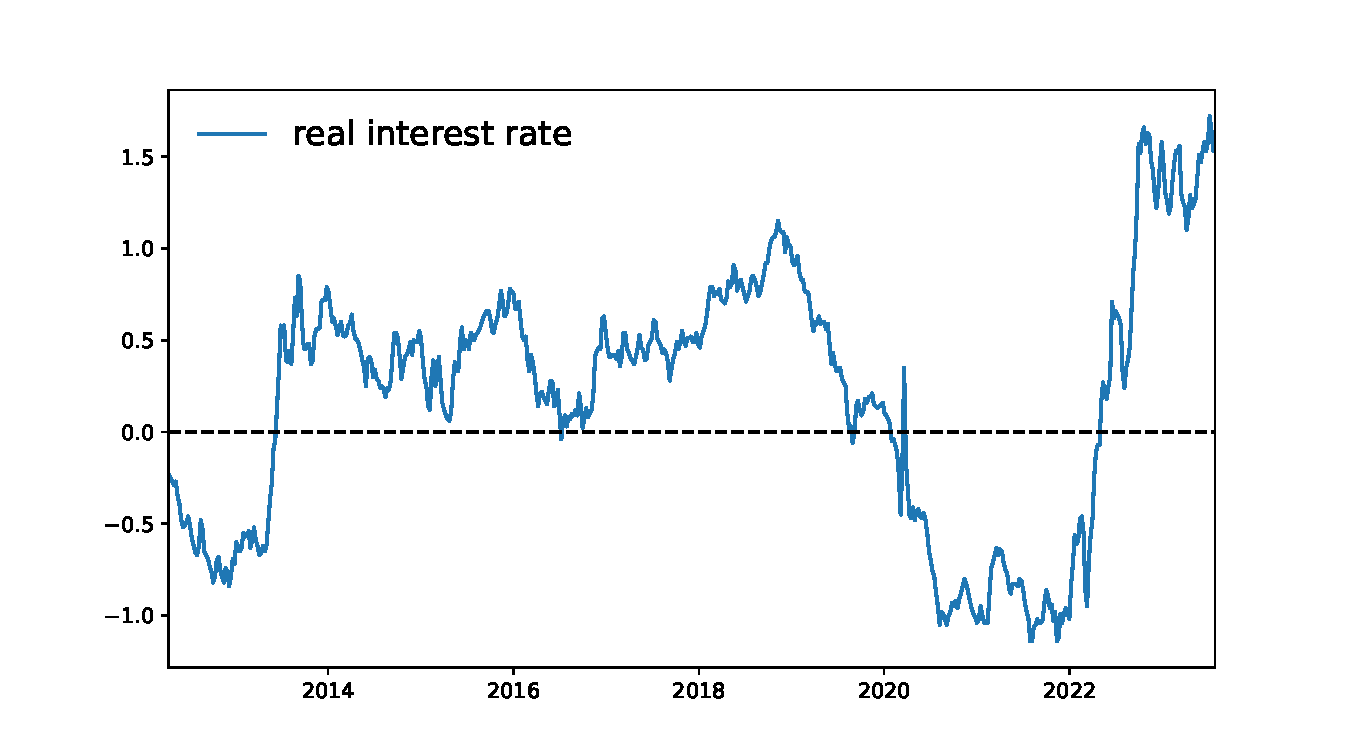
\includegraphics{figures/plot_interest_rates_real.pdf}}
       \caption{\label{f:plot_interest_rates_real} Real US interest rates
           }
    \end{figure}

\end{frame}



\begin{frame}
    
    \Eg \navy{Firm exit with state-dependent discounting}

    \medskip
    \medskip

    The Bellman equation is
    %
    \begin{multline*}
        v(z) =
        \\
        \max_{a \in \{0,1\}}
        \left\{
             a s(z)
             + (1-a) \left[ \pi(z) + \beta(z) \sum_{z'} v(z') P(z, z') \right]
        \right\}
    \end{multline*}
    %
    \medskip

    This is also an affine DP

    %
    \begin{itemize}
        \item $r(z, a) = a s(z) + (1-a)\pi(z)$
        \medskip
        \item $K(z, a, z') = (1 - a) \beta(z) P(z, z')$
    \end{itemize}

\end{frame}

\begin{frame}
    
    \Eg A \navy{shortest path problem} on graph $\gG = (\Xsf, E)$

    \vspace{0.5em}

    \begin{itemize}
        \item $c(x,x') =$ cost of traversing edge $(x,x') \in E$
        \vspace{0.5em}
        \item the direct successors of $x$ denoted by
            %
            \begin{equation*}
                \oO(x) := \setntn{x' \in \Xsf}{(x, x') \in E}   
            \end{equation*}
            %
    \end{itemize}
    

    \vspace{0.5em}
    \vspace{0.5em}
    \vspace{0.5em}
    Aim: find the minimum cost path from $x$ to a specified vertex $d$ 


\end{frame}



\begin{frame}

    The Bellman equation is
    %
    \begin{equation*}
        v(x) = \min_{x' \in \oO(x)} \{ c(x, x') + v(x') \}
    \end{equation*}
    %

    \medskip


    This is an affine DP with 
    %
    \begin{itemize}
        \item state $x \in \Xsf$ and action $a \in \Xsf$
        \medskip
        \item $\Gamma(x) = \oO(x)$ 
        \medskip
        \item $r(x, a) = -c(x, a)$ 
        \medskip
        \item $K(x, a, x') = \1\{x' = a\}$
    \end{itemize}

\end{frame}



\begin{frame}

    \Eg \navy{Inventory management}

    \medskip

    Bellman equation is
    %
    \begin{equation*}
        v(y)
        = \max_{a \in \Gamma(y)} \left\{
            r(y, a)
            + \beta
            \sum_{y'} v(y') R(y, a, y')
        \right\}
    \end{equation*}
    %
    %
    \begin{itemize}
        \item $y \in \{0, \ldots, \bar y\}$ is current inventory 
        \vspace{0.5em}
        \item $a$ is current order (units of stock)
        \vspace{0.5em}
        \item $r(y, a)$ is current profits
        \vspace{0.5em}
        \item $R(y, a, y') =$ prob.\ next state is $y'$ given $y, a$
        \vspace{0.5em}
        \item An affine DP with $K(y, a, y') = \beta R(y, a, y')$
    \end{itemize}



\end{frame}


\begin{frame}
    
    Let's now return to the general case with 
    Bellman equation
    %
    \begin{equation*}
        v(x)
        = \max_{a \in \Gamma(x)}
        \left\{
            r(x, a)
            + \sum_{x'} v(x') K(x, a, x')
        \right\}
    \end{equation*}

    \medskip
    \medskip

    \begin{itemize}
        \item state space is $\Xsf$ (finite)
        \medskip
        \item action space is $\Asf$ (finite)
        \medskip
        \item reward function $r$ maps $\Gsf$ to $\RR$ 
        \medskip
        \item transition kernel $K$ maps $\Gsf \times \Xsf$ to $\RR$ 
    \end{itemize}

\end{frame}

\begin{frame}{Definitions}

    A \navy{feasible policy} is a map $\sigma \colon \Xsf \to \Asf$ with
    %
    \begin{equation*}
        \sigma(x) \in \Gamma(x)
        \quad \text{for all} \quad
        x \in \Xsf
    \end{equation*}

    \begin{itemize}
        \item $\Sigma := $ all feasible policies
    \end{itemize}


    \vspace{0.5em}
    \vspace{0.5em}
    \vspace{0.5em}
    \vspace{0.5em}

    Feasible policy $\sigma$ is called \navy{$v$-greedy} if
    %
    \begin{equation*}
        \sigma(x) \in             
        \argmax_{a \in \Gamma(x)}
        \left\{
            r(x, a)
            + 
            \sum_{x'} v(x') K(x, a, x')
        \right\}
        \quad \forall \, x \in \Xsf
    \end{equation*}

\end{frame}




\begin{frame}
    

    \vspace{0.5em}
    The \navy{Bellman operator} is
    %
    \begin{equation*}
        (Tv)(x)
            = \max_{a \in \Gamma(x)}
            \left\{
                r(x, a)
                + \sum_{x'} v(x') K(x, a, x')
            \right\}
    \end{equation*}

    \vspace{0.5em}
    \vspace{0.5em}
    For each $\sigma \in \Sigma$, we introduce the \navy{policy operator} 
    %
    \begin{equation*}
        (T_\sigma \, v)(x) 
            = r(x, \sigma(x))
            + \sum_{x'} v(x') K(x, \sigma(x), x')
    \end{equation*}


    \vspace{0.5em}
    \vspace{0.5em}

    Note:
    %
    \begin{equation*}
        \sigma \text{ is $v$-greedy}
        \quad \iff \quad
        Tv = T_\sigma \, v
    \end{equation*}

\end{frame}


\begin{frame}

    \begin{figure}
        \centering
        \scalebox{0.5}{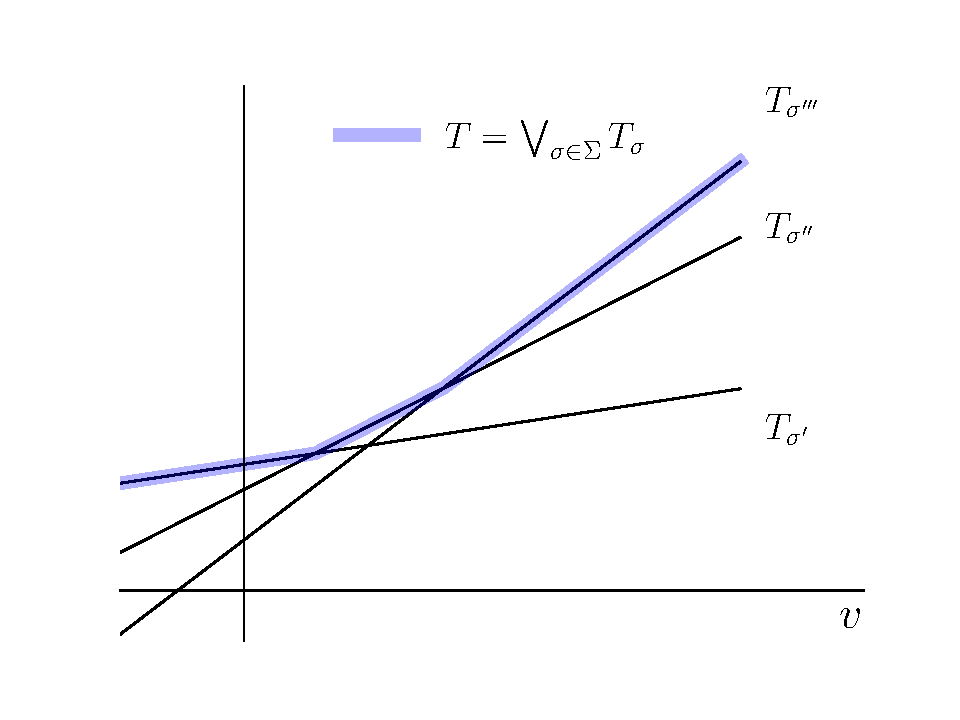
\includegraphics{bellman_envelope.pdf}}
        \caption{\label{f:bellman_envelope} $T$ is the pointwise max.\ of
        $\{T_\sigma\}_{\sigma \in \Sigma}$}
    \end{figure}
    %

\end{frame}


\begin{frame}
    
    Add an intuitive discussion for the recursion that defines $v_\sigma$ in the
    MDP case

\end{frame}


\begin{frame}
    
    Let 
    %
    \begin{itemize}
        \item $r_\sigma(x) := r(x, \sigma(x)) =$  rewards under $\sigma$
        \vspace{0.4em}
        \item $K_\sigma(x, x') := K(x, \sigma(x), x') =$ transitions under
            $\sigma$
    \end{itemize}
        

    The \navy{lifetime value function} associated with policy $\sigma$ is 
    %
    \begin{equation*}
        v_\sigma := (I - K_\sigma)^{-1} r_\sigma
    \end{equation*}

    Note that
    %
    \begin{align*}
        v \in \fix(T_\sigma) 
        & \iff  v  = r_\sigma + K_\sigma v
        \\
        & \iff  (I - K_\sigma) v = r_\sigma
        \\
        & \iff  v = (I - K_\sigma)^{-1}r_\sigma =: v_\sigma
    \end{align*}
    
\end{frame}


\begin{frame}
    \frametitle{Defining optimality}
    
    We define the \navy{value function}  via
    
    \begin{equation*}
        v^*(x) := \max_{\sigma \in \Sigma} v_\sigma(x)
        \quad \qquad (x \in \Xsf)
    \end{equation*}

    \vspace{0.4em}
    \vspace{0.4em}

    Equivalently,
    %
    \begin{equation*}
        v^* := \bigvee_\sigma v_\sigma
    \end{equation*}

    \vspace{0.4em}
    \vspace{0.4em}
    \vspace{0.4em}
    \vspace{0.4em}
    A policy $\sigma$ is called \navy{optimal} if $v_\sigma = v^*$


\end{frame}




\begin{frame}
    \frametitle{MDP Optimality}

    \begin{block}{\vspace*{-3ex}}
        {\bf Theorem.} For an MDP with Bellman operator
        $T$ and value function $v^*$,
            \vspace{0.5em}
        %
        \begin{enumerate}
            \item $v^*$ is the unique fixed point of $T$
                in $\RR^\Xsf$
            \vspace{0.5em}
            \vspace{0.5em}
            \item $T$ is a contraction mapping on $\RR^\Xsf$
            \vspace{0.5em}
            \vspace{0.5em}
            \item A feasible policy is optimal if and only it is $v^*$-greedy
            \vspace{0.5em}
            \vspace{0.5em}
            \item At least one optimal policy exists
        \end{enumerate}
        %
    \end{block}


\end{frame}

\begin{frame}
    
    Standard algorithms

\end{frame}

\begin{frame}

    {\small 
        \begin{algorithm}[H]
        \DontPrintSemicolon
        \vspace{0.2em}
        input $v_0 \in \RR^\Xsf$ \;
        \vspace{0.2em}
        input $\tau$, a tolerance level for error \;
        \vspace{0.2em}
        $\epsilon \leftarrow +\infty$ \;
        \vspace{0.2em}
        $k \leftarrow 0$ \;
        \vspace{0.2em}
        \While{$\epsilon > \tau $}
        {
        \vspace{0.2em}
            $v_{k+1} \leftarrow Tv_k$ \;
            \vspace{0.2em}
            $\epsilon \leftarrow \| v_k - v_{k+1} \|_\infty$ \;
            \vspace{0.2em}
            $k \leftarrow k + 1$ \;
        \vspace{0.2em}
        }
        \vspace{0.2em}
        Compute a $v_k$-greedy policy $\sigma$ \;
        \vspace{0.2em}
        \Return{$\sigma$}
        \vspace{0.2em}
        \caption{VFI}
        \end{algorithm}
    }


\end{frame}



\begin{frame}
    

    \begin{algorithm}[H]
        \DontPrintSemicolon
        \vspace{0.5em}
        input $\sigma_0 \in \Sigma$, set $k \leftarrow 0$ and $\epsilon \leftarrow 1$ \;
        \vspace{0.5em}
        \While{$\epsilon > 0 $}
        {
            $v_k \leftarrow $ the lifetime value of $\sigma_k$ \;
        \vspace{0.5em}
            $\sigma_{k+1} \leftarrow $ a $v_k$-greedy policy \;
        \vspace{0.5em}
            $\epsilon \leftarrow \1\{ \sigma_k \not= \sigma_{k+1} \}$ \;
        \vspace{0.5em}
            $k \leftarrow k + 1$ \;
        }
        \vspace{0.5em}
        \Return{$\sigma_k$}
        \caption{HPI}
    \end{algorithm}

\end{frame}



\begin{frame}
    
    \begin{figure} 
        \centering
        \scalebox{0.48}{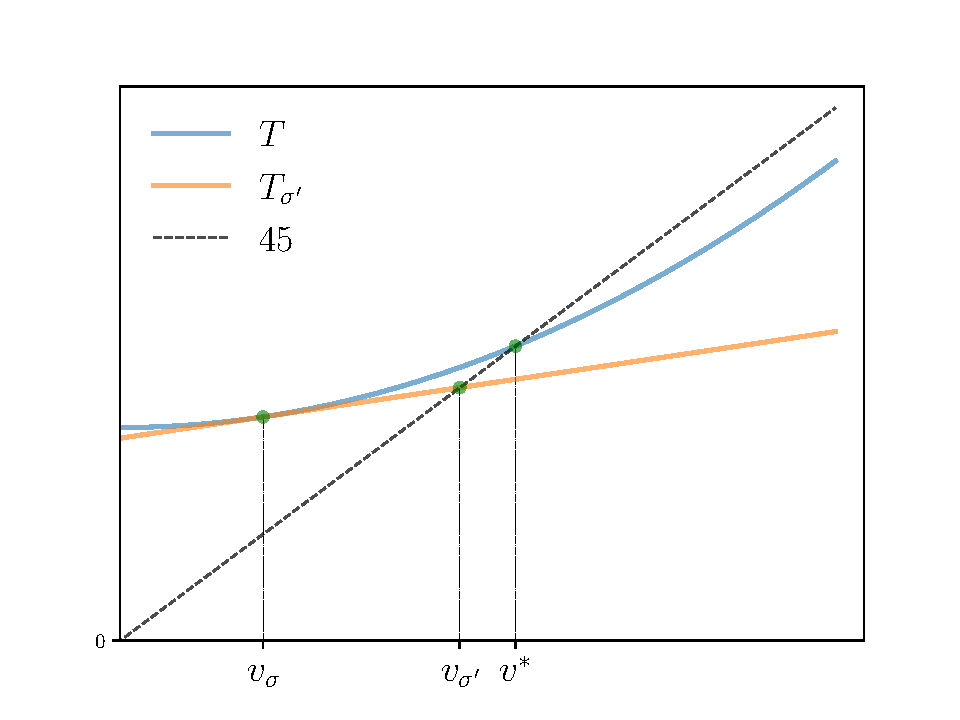
\includegraphics{howard_newton_1.pdf}}
        \caption{\label{f:howard_newton_1} HPI as a version of Newton's method}
    \end{figure}
    %

\end{frame}


\begin{frame}
    
    {\small
    \begin{algorithm}[H]
        \DontPrintSemicolon
        \vspace{0.2em}
        input $v_0$, an initial guess of $v^*$ \;
        \vspace{0.2em}
        input $\tau$, a tolerance level for error \;
        \vspace{0.2em}
        input $m \in \NN$, a step size \;
        \vspace{0.2em}
        $k \leftarrow 0$ \;
        \vspace{0.2em}
        $\epsilon \leftarrow +\infty$ \;
        \vspace{0.2em}
        \While{$\epsilon > \tau $}
        {
            \vspace{0.2em}
            $\sigma_k \leftarrow $ a $v_k$-greedy policy \;
            \vspace{0.2em}
            $v_{k+1} \leftarrow T_{\sigma_k}^m v_k$  \;
            \vspace{0.2em}
            $\epsilon \leftarrow \| v_k - v_{k+1} \|_\infty$ \;
            \vspace{0.2em}
            $k \leftarrow k + 1$ \;
            \vspace{0.2em}
        }
        \Return{$\sigma_k$}
        \vspace{0.2em}
        \caption{OPI}
    \end{algorithm}
    }

\end{frame}


\begin{frame}
    
    \vspace{0.4em}
    \vspace{0.4em}
    \vspace{0.4em}
    \begin{block}{\vspace*{-3ex}}
    {\bf Proposition.} Under the stated condition, VFI, HPI and OPI all converge
    \vspace{0.4em}
    \vspace{0.4em}

    Moreover, HPI converges to an exact optimal policy in finitely many steps
    \end{block}


    \vspace{0.4em}
    \vspace{0.4em}
    For details and proofs see Ch.\ 5 of \url{https://dp.quantecon.org/}


\end{frame}


\end{document}









